


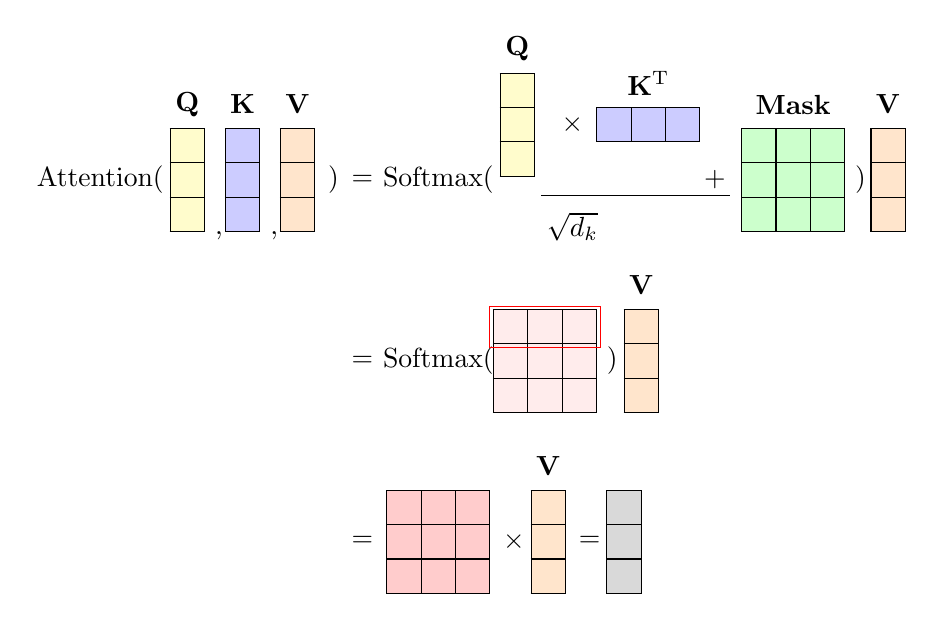
\begin{tikzpicture}
\node(atten) at (0,0){Attention(};
%%%% Q
\node(tbq) at ([xshift=0.5em,yshift=0]atten.east){
\begin{tabular}{|c|}
\hline
\rowcolor{yellow!20}  \\ \hline 
\rowcolor{yellow!20}  \\ \hline
\rowcolor{yellow!20}  \\ \hline 
\end{tabular}
};
\node at  ([xshift=0em,yshift=0.5em]tbq.north){$\mathbf{Q}$};

\node(comma1) at ([xshift=0.15em,yshift=-2em]tbq.east){,};

%%%% k
\node(tbk) at ([xshift=1em,yshift=0]tbq.east){
\begin{tabular}{|c|}
\hline
\rowcolor{blue!20}  \\ \hline 
\rowcolor{blue!20}  \\ \hline
\rowcolor{blue!20}  \\ \hline 
\end{tabular}
};
\node at  ([xshift=0em,yshift=0.5em]tbk.north){$\mathbf{K}$};

\node(comma2) at ([xshift=0.15em,yshift=-2em]tbk.east){,};

%%%% v
\node(tbv) at ([xshift=1em,yshift=0]tbk.east){
\begin{tabular}{|c|}
\hline
\rowcolor{orange!20}  \\ \hline 
\rowcolor{orange!20}  \\ \hline
\rowcolor{orange!20}  \\ \hline 
\end{tabular}
};
\node at  ([xshift=0em,yshift=0.5em]tbv.north){$\mathbf{V}$};

\node(bra) at ([xshift=0.3em,yshift=0]tbv.east){)};

\node(eq1) at ([xshift=0.5em,yshift=0]bra.east){=};

\node(sof1) at ([xshift=2em,yshift=0]eq1.east){Softmax(};

%-----------------------------------------------------------
%QK+MASK
\node(tbq2) at ([xshift=0.5em,yshift=2em]sof1.east){
\begin{tabular}{|c|}
\hline
\rowcolor{yellow!20}  \\ \hline 
\rowcolor{yellow!20}  \\ \hline
\rowcolor{yellow!20}  \\ \hline 
\end{tabular}
};
\node at  ([xshift=0em,yshift=0.5em]tbq2.north){$\mathbf{Q}$};


% x
\node (times) at  ([xshift=1em,yshift=0em]tbq2.east){$\times$};

%k
\node(tbk2) at ([xshift=2em,yshift=0em]times.east){
\begin{tabular}{|l|l|l|}
\hline
\cellcolor{blue!20} & \cellcolor{blue!20} &\cellcolor{blue!20}  \\ \hline
\end{tabular}
};
\node at  ([xshift=0em,yshift=0.5em]tbk2.north){$\mathbf{K}^{\mathrm{T}}$};

\draw [-] (5.6,-0.2) -- (8,-0.2);

\node at  ([xshift=0em,yshift=-3em]times.south){$\sqrt{d_k}$};
% MASK
\node(mask) at  ([xshift=3em,yshift=-2em]tbk2.east){
\begin{tabular}{|l|l|l|}
\hline
\cellcolor{green!20} &\cellcolor{green!20}   &\cellcolor{green!20}   \\ \hline
 \cellcolor{green!20} &\cellcolor{green!20}   &\cellcolor{green!20}   \\ \hline
 \cellcolor{green!20} &\cellcolor{green!20}   &\cellcolor{green!20}   \\ \hline
\end{tabular}
};
\node at  ([xshift=0em,yshift=0.5em]mask.north){$\mathbf{Mask}$};
%+
\node at  ([xshift=-0.6em,yshift=0em]mask.west){$+$};
%)
\node at  ([xshift=0.2em,yshift=0em]mask.east){)};

%%%% v
\node(tbv2) at ([xshift=1.2em,yshift=0]mask.east){
\begin{tabular}{|c|}
\hline
\rowcolor{orange!20}  \\ \hline 
\rowcolor{orange!20}  \\ \hline
\rowcolor{orange!20}  \\ \hline 
\end{tabular}
};
\node at  ([xshift=0em,yshift=0.5em]tbv2.north){$\mathbf{V}$};

%------------------------------
%第二行
\node(eq2) at  ([xshift=0em,yshift=-6em]eq1.south){=};
\node(sof2) at ([xshift=2em,yshift=0]eq2.east){Softmax(};
%中间粉色矩阵
\node(mid) at  ([xshift=1.5em,yshift=0em]sof2.east){
\begin{tabular}{|l|l|l|}
\hline
\cellcolor{pink!30} &\cellcolor{pink!30}   &\cellcolor{pink!30}   \\ \hline
 \cellcolor{pink!30} &\cellcolor{pink!30}   &\cellcolor{pink!30}   \\ \hline
 \cellcolor{pink!30} &\cellcolor{pink!30}   &\cellcolor{pink!30}   \\ \hline
\end{tabular}
};
% )
\node(bra2) at ([xshift=0.2em,yshift=0]mid.east){)};
%红色框
\node[rectangle,minimum width=4.0em,minimum height=1.5em,draw=red](p222) at([xshift=0em,yshift=-1.0em]mid.north) {};

%%%% v
\node(tbv3) at ([xshift=0.5em,yshift=0]bra2.east){
\begin{tabular}{|c|}
\hline
\rowcolor{orange!20}  \\ \hline 
\rowcolor{orange!20}  \\ \hline
\rowcolor{orange!20}  \\ \hline 
\end{tabular}
};
\node at  ([xshift=0em,yshift=0.5em]tbv3.north){$\mathbf{V}$};

%------------------------------------
%第三行
\node(eq3) at  ([xshift=0em,yshift=-6em]eq2.south){=};
%%%% softmax结果 红色矩阵
\node(result) at ([xshift=2em,yshift=0]eq3.east){
\begin{tabular}{|l|l|l|}
\hline
\cellcolor{red!20} &\cellcolor{red!20}   &\cellcolor{red!20}   \\ \hline
\cellcolor{red!20}&\cellcolor{red!20}   &\cellcolor{red!20}   \\ \hline
\cellcolor{red!20} &\cellcolor{red!20}  &\cellcolor{red!20}   \\ \hline
\end{tabular}
};
% x
\node (times) at  ([xshift=0.5em,yshift=0em]result.east){$\times$};
%%%% v
\node(tbv4) at ([xshift=0.5em,yshift=0]times.east){
\begin{tabular}{|c|}
\hline
\rowcolor{orange!20}  \\ \hline 
\rowcolor{orange!20}  \\ \hline
\rowcolor{orange!20}  \\ \hline 
\end{tabular}
};
\node at  ([xshift=0em,yshift=0.5em]tbv4.north){$\mathbf{V}$};
%=
\node(eq4) at  ([xshift=0.5em,yshift=0em]tbv4.east){=};

%%%% 灰色矩阵
\node(gre) at ([xshift=0.5em,yshift=0]eq4.east){
\begin{tabular}{|c|}
\hline
\rowcolor{black!15}  \\ \hline 
\rowcolor{black!15}  \\ \hline
\rowcolor{black!15}  \\ \hline 
\end{tabular}
};

\end{tikzpicture}